\chapter{Autobahn}
%\corner{64}
\vepsianrose
%\fancyhead[LE]{\fancyplain{}{\bfseries \parttitle}}
%\fancyhead[RO]{\fancyplain{}{\bfseries \rightmark}}

Шурик, облачённый в штормовку, сидел в машине, на~улице собирался дождь. Утро старта, наконец\sdash то! Багажник был почти под завязку\mdash упакованная байдарка занимала дочерта места, пришлось сложить половину заднего ряда сидений. Мыслей как будто бы не было, он парил где\sdash то в неведомых облаках, преображаясь в своём сознании в Адмирала Сплава. Ему с одной стороны было как\sdash то некомфортно и~даже стыдно оставлять жену с~ребёнком одних дома, а~самому отправляться в~путешествие, а~с~другой стороны он понимал, что жить не~может уже без реки, тем более он не был в~походе целых три года. В своём сознании Шурик был до~предела измотан всем, всем, что его окружало\mdash грёбаными электричками, работой, семьёй, медиапространством и вообще всем плохим, что произошло в мире, стране и в целом в его жизни за~последние 2\thinspace\nobreakdash---\thinspace3 года. И~эти десять дней, на которые он вырывается из~всего этого, были для него как глоток свежего воздуха, как припадение к чистейшему горному роднику, как некий абсолют желаний задолбавшегося человека\mdash не видеть вокруг себя толпы людей из транспорта и тихо заниматься простыми древними вещами\mdash разводить огонь, готовить еду, плыть по реке$\ldots$ Очнувшись, Адмирал глянул на~часы\mdash пора! Он повернул ключ зажигания, завёл машину, вбил в~навигаторе адрес Кири, написал тому, что выехал, и нажал на~газ. Заброска началась.

Спустя полчаса он очень удачно запарковался аккурат перед подъездом Кири, тот вышел c баулами буквально через пару минут.

\diagdash Кирь, опять вещей\mdash мама дорогая!

\diagdash Не гунди, Шурик, щас ещё пару вещмешков.\mdash они грузились под накрапывавшим дождичком, который как всегда так невовремя начался.

\diagdash Тебе помочь?

\diagdash Не, сам$\ldots$\mdash Замполит пошёл за очередными баулами.

\diagdash Ладно, жене привет.

Безумно хотелось закурить, но Адмирал не поддался соблазну, обошёл кругом машину и сел за руль. Занавеска на кирином балконе подёрнулась\mdash жена подошла к~окну проводить Кирю. Вскоре тот семимильными шагами стремительно вышел из подъезда, запихал последнюю герму в багажник и, захлопнув его, плюхнулся на~переднее пассажирское:

\diagdash Ну чё, погнали?

\diagdash Попрощался? Погнали$\ldots$

\diagdash От винта!

\renewcommand*{\thefootnote}{\arabic{footnote}}
%\renewcommand*{\thefootnote}{\fnsymbol{footnote}}

Дождь усиливался. Уже когда друзья оказались на~МКАДе\footnote{Московская кольцевая автомобильная дорога.}, зарядил настоящий ливень. Погода обильно, не щадя, омывала друзей водными потоками, приветствуя таким образом стартующих сплавщиков. Теперь они\mdash больше не Шурик и Киря, а Адмирал и Замполит Сплава, они вновь собрались вместе, а значит их байдарки вновь рассекут водную гладь, вновь вода будет повсюду, а~пьянящая хмельная свобода просторов родной страны подлечит душевные раны.

\diagdash Вы умеете выбрать погодку, тащ Адмирал!\mdash задумчиво произнёс Замполит, глядя в окно на дождь.

\diagdash Так, ля, Замполит! Срочно звони Роман Менделичу\footnote{Роман Менделевич Вильфанд\mdash метеоролог, директор <<Гидрометцентра России>>.}, договаривайся там, короче, делай шо хош, чтоб погодка была тип\sdash топ!

\diagdash Не иначе! Приколи под таким дождём плыть 7 дней?

\diagdash Не накаркай$\exldots$

\vspace{0.5cm}
$\ldots$Друзья подкатили во двор пашкиного дома и~перегрузили шмот из его машины в шурикову:

\diagdash Пацаны, столько шмотья, по\sdash моему компоты где\sdash то здесь, а бензопилу не взяли!\mdash иронизировал Паша.\mdash Мне~ж~совсем места не останется!

\diagdash Так, давай по-другому распихаем$\ldots$

\diagdash Как ни распихивай, уже под потолок барахла!

Старательно утрамбовав снарягу, сплавщики наконец\sdash то выехали из Москвы и вырулили на платную питерскую трассу М\sdash11\mdash Шурик незадолго до сплава приобрёл транспондер для бесконтактной оплаты проезда.

\diagdash Замполит, набери Серёге, где они там?\mdash попросил Адмирал узнать что там со вторым экипажем.

\diagdash Момент$\ldots$

Оказалось, что Серёга с Русланом ехали практически параллельно им, но по обычной, бесплатной, дороге. По~расчётам Адмирала выходило, что разница в их прибытии в~Старую Ладогу составит от 40 минут до часа.

Троица проехала пункт оплаты, где транспондер, пикнув, открыл им шлагбаум. Дорога была шикарна\mdash как масло. Адмирал бодро рванул вперёд по автостраде, утапливая педаль газа в~пол и~поздно переключаясь на~повышенную передачу, отчего движок знавшего и лучшие годы 10\sdash летнего седана гулко выл:

\diagdash Эй, блин, я хочу живым домой вернуться!\mdash отвлёкся Киря от телефона.

\setcounter{footnote}{0}
\renewcommand*{\thefootnote}{\arabic{footnote}}
%\renewcommand*{\thefootnote}{\fnsymbol{footnote}}

\diagdash Не очкуй, аллес унтер контролле\footnote{Всё под контролем (нем. alles unter Kontrolle).}!\mdash отозвался Адмирал.\mdash Руссише аутобанен приветствуют вас! За~бортом +22 градус\'{а} выше н\'{о}ля, полёт проходит норм\'{у}льно, расчётное время прибытия\mdash айн унд цв\'{а}нцихъ\footnote{Двадцать один (нем. einundzwanzig).} ч\'{а}сен ровно. В полёте вам будут предложены напитки и бутерброды.

\diagdash Да?! Это где?\mdash поинтересовался Паша, не взявший с собой перекуса.

\diagdash На заправке! Ы-ы-ы!

%\makebox[\linewidth][s]{Дождь помаленьку прекращался по мере их}
%Дождь помаленьку прекращался по мере их удаления от Москвы.
%Дождь помаленьку прекращался по мере их
\makebox[\linewidth-\parindent][s]{Дождь помаленьку прекращался по мере их}

\newpage

{
\setlength{\belowcaptionskip}{-5mm}
\begin{figure}[h]
	\centering
	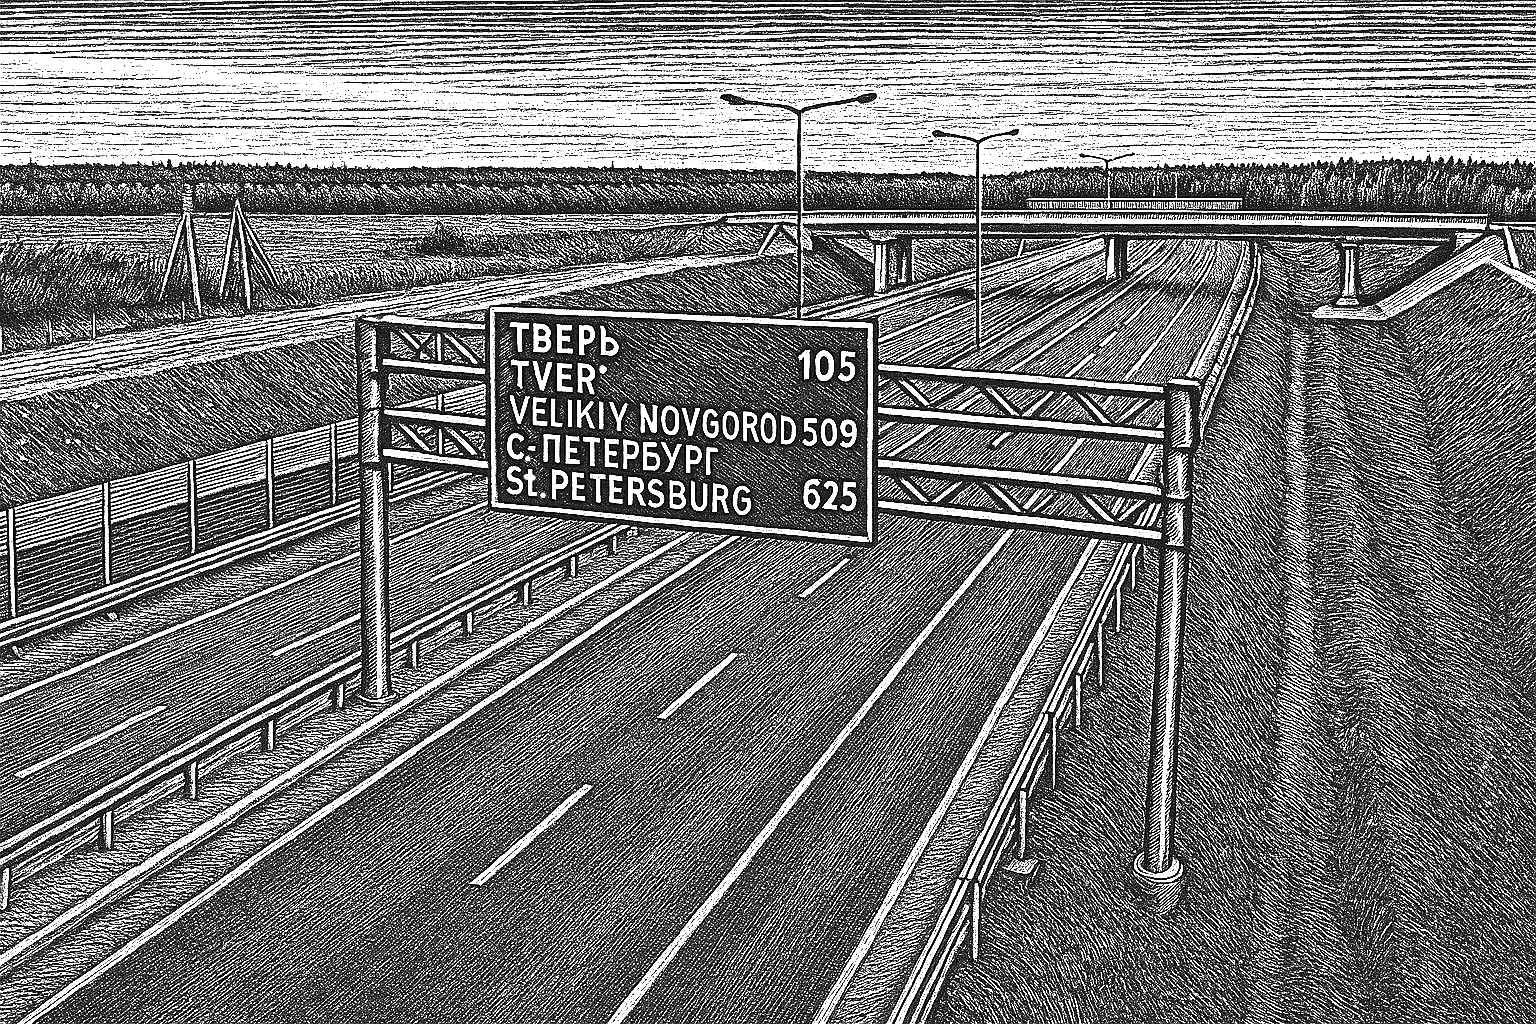
\includegraphics[width=1.0\textwidth]{06_1_highway}
	\caption{\small\textit{...бодро рванул вперёд по автостраде, утапливая педаль газа...}}
\end{figure}

\noindent удаления от Москвы. Трасса была мокрой, поэтому Адмирал всё же не лихачил. За трёпом потихоньку долетели до Твери, где заправились бензом и перекусили на заправке:
}

\diagdash Лишь бы не как в прошлый раз с погодой.\mdash изрёк Паша, доедая бутерброд.

\diagdash Да всё наладится! Смотри, уже и дождя нет, щас солнце выглянет!\mdash потягивал Замполит кофе с сигареткой.

После заправки парни сели на хвост какому\sdash то резвому водителю и~в~таком режиме допилили до съезда с платной М\sdash 11 на старую питерскую трассу М\sdash10, с которой они вскоре свернули после Чудово. Адмирал порядком притомился за~рулём, потому что поддержание высокоскоростного режима требовало и высокой концентрации внимания. И~тут~Замполит~внезапно~выпалил:

\diagdash ШУРИК! Едем обратно!!!

\diagdash Утюг не выключил?\mdash лениво ввернул Адмирал.

\diagdash ХУЖЕ!!! Я забыл ложку и миску свои титановые!

%\diagdash Кирь, ну всё, придется жменькой суп хлебать или того хуже\mdash как простые смертные, из нержавейки.
\diagdash Кирь, ну всё, придётся хлебать суп как простые смертные\mdash из нержавейки.

\diagdash Шурик, катастрофа, я собирался, собирался, вот как чувствовал, что забыл что\sdash то, и вот тебе раз! Мой тита\sdash а\sdash ан!

\diagdash Забей, чё там дальше по карте?

\diagdash Ща гляну$\ldots$\mdash Замполит уткнулся в карту.\mdash Кириши какие\sdash то$\ldots$

\diagdash А? КирЮши?

\diagdash Ки-ри-ши, тащ Адмирал. Там и спортивный есть.

\diagdash А ты думал? Растёт благосостояние народа! В~КирЮшах есть спортивный магазин, никогда бы не~подумал.\mdash вовсю иронизировал тот.

\diagdash А давайте в Киришах где\sdash нить покушаем нормально,~а?\mdash отозвался с~заднего сиденья Паша.

\diagdash Лад\'{ы}! Кирь, выбери там чё нить?

И Замполит проложил по~навигатору ответвление с~маршрута в эти самые Кириши, которые вскоре показались после очередного поворота. Отзвонился Серёга\mdash они плелись далеко позади на М\sdash 10:

\diagdash Пацаны, Руслан кружку забыл!

\diagdash Классика! Купим ему, мы как раз в спортивный щас заедем\mdash Киря тоже забыл!

%\renewcommand*{\thefootnote}{\arabic{footnote}}
\renewcommand*{\thefootnote}{\fnsymbol{footnote}}
\setcounter{footnote}{0}
\diagdash Прикол! Ладно, мы тут пока в пробках чилим\footnote{Ч\'{и}лить (от англ. chill\mdash прохлаждаться)\mdash расслабленно отдыхать.}$\ldots$

Киря, Шурик и Паша запарковались у спортивного и достаточно быстро прикупили всё, что забыли\mdash благосостояние народа таки растёт. А потом, перекусив в~общепите, немного передохнули и снова двинулись в путь\mdash до Старой Ладоги оставалось совсем немного, порядка 60~километров.

И вот, спустя где\sdash то час, который прошёл относительно спокойно\mdash на трассе местного значения\mdash друзья проехали Волхов, где ужасным дымом смердило множество труб заводов. Совсем скоро после этого показалась и~Старая Ладога, их конечная точка на сегодня. Уже стемнело, когда путешественники проехали мимо Староладожской крепости, которую хотели завтра посетить. Она подсвечивалась в ночи прожекторами и выглядела монументально, величественно. Как будто хоть сейчас из её ворот готова была показаться княжеская конная дружина. Высокие крепостные стены и~башни, покрытые сверху деревянными конусами, смотрелись ну просто великолепно\mdash Шурику всегда нравилась такая архитектура, и сейчас он, даже на~мгновение оторвав взгляд от дороги на крепость, ощутил прилив позитива. 

Команда проехала дальше и~свернула к гостинице, во дворе которой они запарковались в 21:30, разойдясь с расчётным временем прибытия всего на~полчаса\mdash нормально, с учётом того, что ещё заезжали в~Кириши.

\diagdash Так, пацаны, я в магаз!\mdash огласил Паша, вылезая из~машины.\mdash Сил нету!

\diagdash Пошли!

Вскоре друзья расположились на балкончике номера, задымили и, откинувшись на табуреточках, с~наслаждением прихлебнули светлого, наблюдая вдалеке над лесом восход полной Луны. Прошло около часа, пацаны чилили на~балконе, болтая о всякой ерунде:

\diagdash Полнолу\sdash у\sdash уние! Всякая не\sdash е\sdash ечисть вылезает из~угло\sdash о\sdash ов! Вурдалаки и русалки подстерегают пу\sdash у\sdash утников, забредших в неведомые дали!!!\mdash заворачивал Шурик.

\diagdash Хар\'{о}ш! Смотри, чтоб из матраса твоего нечисть не~вылезла!\mdash сказал вошедший в комнату Серёга и~стал, приподняв и перевернув матрас, пристально осматривать место ночёвки на предмет клопов. Друзья и не заметили как подрулила вторая часть команды.

\diagdash Ну как? Есть тараканчики?\mdash лениво протянул Шурик.

\diagdash Да вроде нет$\ldots$ Ну и дыру ты выбрал на ночёвку! 

\diagdash Забей, нам просто поспать. Другое всё было или занято или сильно дороже. Выдыхай, мы тут всего до утра.

Серёга представил команде Руслана, все перезнакомились, тут же закрепив это чарочкой пенного, а после продолжили посиделки и прочий трёп, который, впрочем, достаточно скоро стих, и в комнате раздался чей\sdash то раскатистый храп. Шурик сквозь сон подумал, что лишь бы это не Киря, ведь в сплаве им делить одну палатку на двоих.

\vspace{-0.2cm}
\begin{center}
	\psvectorian[scale=0.4]{88} % Красивый вензелёк :)
\end{center}